\documentclass[10pt]{beamer}

\usepackage[T1]{fontenc}

\usepackage{mathtools}
\usetheme{Montpellier}
\usepackage{tipa}
\usepackage{silence,lmodern}
\usepackage[backend=biber, style=ieee]{biblatex}
\usepackage{minted}
\usepackage{seqsplit}
\hypersetup{colorlinks = true, urlcolor=blue, linkcolor=black}

\WarningFilter{biblatex}{Patching footnotes failed}

\renewcommand*{\bibfont}{\tiny}

\bibliography{resources.bib}

\title{\textbf{Operating Systems}}
\subtitle{Tutorial}
\date{Week 1}

\begin{document}

\frame{\titlepage}

\begin{frame}
  \frametitle{TOC}
  \tableofcontents[hideallsubsections]
\end{frame}
%% Check TUM Aufgaben

\begin{frame}{Intro}
\begin{itemize}
 \item Problems with sheet 0?
 \item Did someone install Arch Linux?
 \item Did you test your C toolchain?
 \item Other issues?
\end{itemize}
\end{frame}

\section{Submission \& git}
    \frame{\sectionpage}
    \begin{frame}{Submission}
        \begin{itemize}
        \item Submissions by everybody on her/his own
        \item Teamwork is allowed, \alert{copy-pasting is not allowed!}
        \item If you plagiarize, you get no points.
        \item use the folder to submit (note to self: show it)
        \end{itemize}
    \end{frame}
    
    \begin{frame}[fragile]{Settings}      
     \begin{itemize}
      \item Once: Go to settings $\rightarrow$ visibility and set \\
      \alert{Project Visibility $\rightarrow$ Private} \vspace{0.2cm} \\
      \item Once: Add the base repository as upstream: \vspace{0.2cm} \\
           \begin{minted}[fontsize=\footnotesize,breaklines,autogobble]{bash}
        git remote add upstream git@gitlab.inf.uni-konstanz.de:matthias.rupp/betriebssysteme.git
      \end{minted} 
      \vspace{0.2cm}
              \end{itemize}
      \end{frame}
      
      \begin{frame}[fragile, allowframebreaks]{basic git commands}
      \begin{itemize}
      \item List all associated remotes \mintinline{bash}{git remote -v}
      
      \item Update from the base repository:
      \begin{minted}[fontsize=\footnotesize,breaklines,autogobble]{bash}
        git fetch upstream
        git merge upstream/master
        git commit -am "merge updates"
        git push
      \end{minted}
      
      \item Update from your own repository \mintinline{bash}{git pull}

      \item Submit you work: \\
      \begin{minted}[fontsize=\footnotesize,breaklines,autogobble]{bash}
       git add <folders and files>
       git commit -m "<message>"
       git push
      \end{minted}

        \framebreak
    
      \item Undo a commit without changing the files locally \mintinline{bash}{git reset --soft HEAD~1}
      
      \item Reset your repository to the state of the latest commit \mintinline{bash}{git reset --hard HEAD~1}
 
      \item Squashing 3 commits together \mintinline{bash}{git rebase -i HEAD~3} and then select squash on all but the most recent commit.
      
      \item Show the differences between the last two commits \mintinline{bash}{git diff HEAD HEAD~1}
      
      \item Show the log of commits \mintinline{bash}{git log}
      
      \item Search text in files under version control \mintinline{bash}{git grep}
      \item substitute commit hash instead of HEAD
      \end{itemize}
      \framebreak
      \begin{figure}
       \begin{center}
       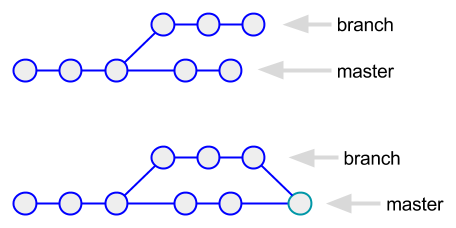
\includegraphics[keepaspectratio, width=\textwidth,height=0.9\textheight-4\baselineskip]{img/001_git-branching.png}
      \end{center}
      \caption{Git branching workflow~\autocite{dzone}}
      \end{figure}
      \framebreak
      \begin{itemize}
      \item List existing branches \mintinline{bash}{git branch -v}
      \item Switch branches \mintinline{bash}{git checkout <branch>}
      \item Create and switch to a new branch \mintinline{bash}{git checkout -b <branch name>}
      \item Delete branch locally \mintinline{bash}{git branch -d <branch name>}
      
      \item Delete branch from remote \mintinline{bash}{git push origin --delete <branch>}
      
     \end{itemize}
      \framebreak
      \begin{figure}
       \begin{center}
       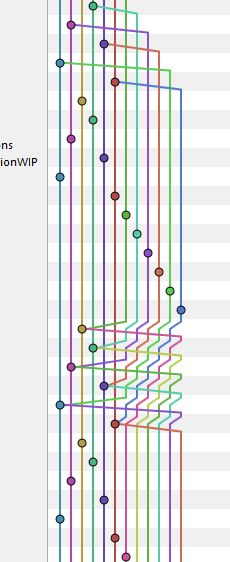
\includegraphics[keepaspectratio, width=\textwidth,height=0.9\textheight-4\baselineskip]{img/001_git_fuckup.png}
      \end{center}
      \caption{``I fucked up Git so bad it turned into Guitar Hero.''~\autocite{twitter}}
      \end{figure}
    \end{frame}
    
\section{Quick Lecture Recap}
\frame{\sectionpage}
\subsection{Overview}
\begin{frame}{Definition}
\begin{figure}
       \begin{center}
       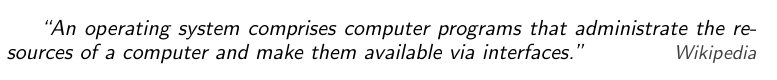
\includegraphics[keepaspectratio, width=\textwidth,height=0.9\textheight-4\baselineskip]{img/100_definition.png}
      \end{center}
      \caption{The defintion given by Wikipedia.~\autocite{wiki}}
      \end{figure}
\end{frame}

\begin{frame}{Overview}
\begin{figure}
       \begin{center}
       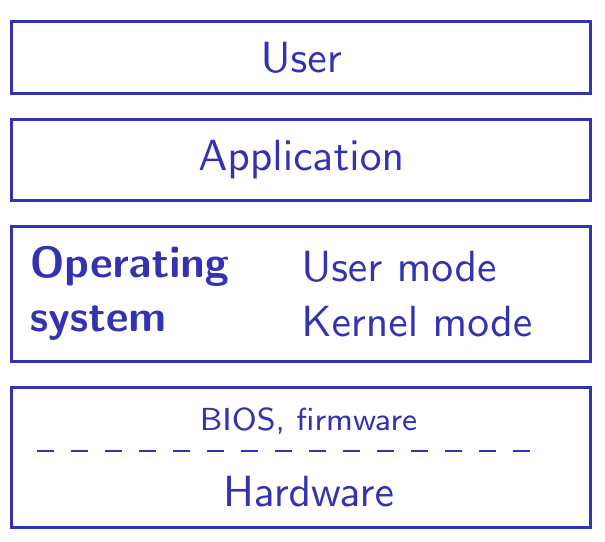
\includegraphics[keepaspectratio, width=\textwidth,height=0.9\textheight-4\baselineskip]{img/101_overview.png}
      \end{center}
      \caption{High level view on an OS.~\autocite{mrupp}}
      \end{figure}
\end{frame}

\begin{frame}{High-level Requirements}
\begin{figure}
       \begin{center}
       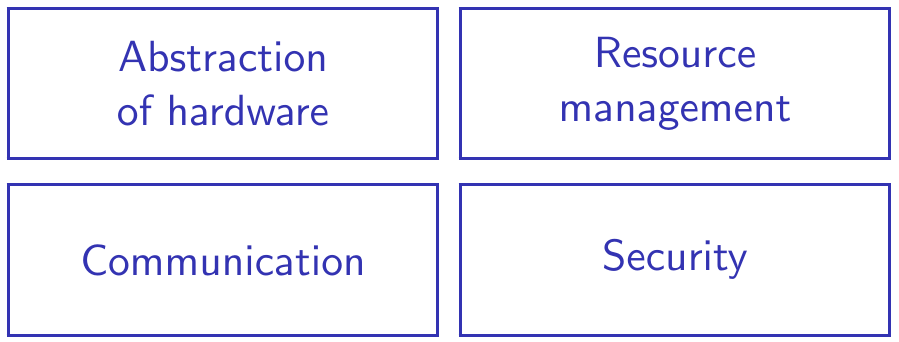
\includegraphics[keepaspectratio, width=\textwidth,height=0.9\textheight-4\baselineskip]{img/102_tasks.png}
      \end{center}
      \caption{High-level requirements of an operating system.~\autocite{mrupp}}
      \end{figure}
\end{frame}

\begin{frame}{Topics}
\begin{figure}
       \begin{center}
       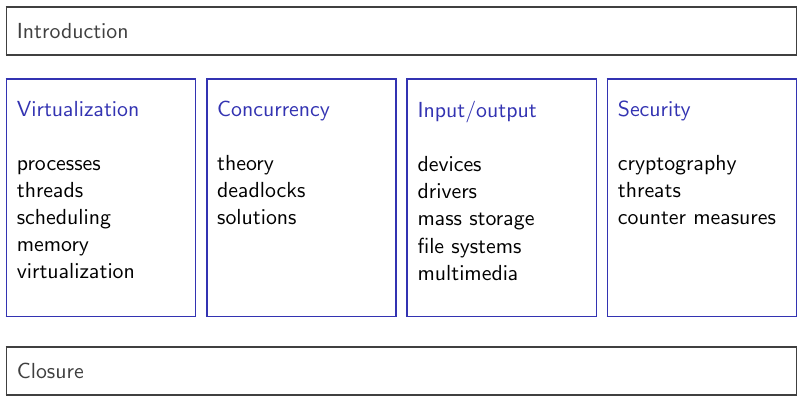
\includegraphics[keepaspectratio, width=\textwidth,height=0.9\textheight-4\baselineskip]{img/103_schedule.png}
      \end{center}
      \caption{Conceptual schedule of the course.~\autocite{mrupp}}
      \end{figure}
\end{frame}

\begin{frame}{Operating System Types}
Custom OSes
\begin{itemize}
 \item Robotics (e.g. \ for Mars Rovers)
 \item Automated Manufacturing 
 \item Gaming Consoles (e.g. Playstation)
\end{itemize}

\begin{figure}
       \begin{center}
       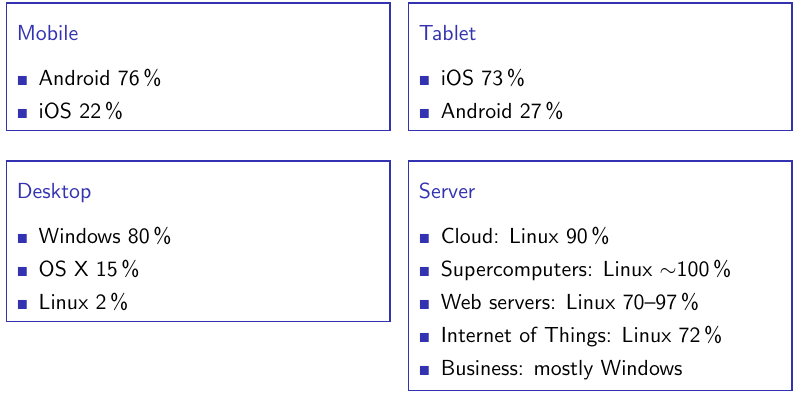
\includegraphics[keepaspectratio, width=\textwidth,height=0.7\textheight-4\baselineskip]{img/104_market_share.png}
      \end{center}
      \caption{Market share of broadband OS use cases.~\autocite{mrupp}}
      \end{figure}
\end{frame}

\subsection{Hardware}
\begin{frame}{Computing Architectures}
\begin{figure}
       \begin{center}
       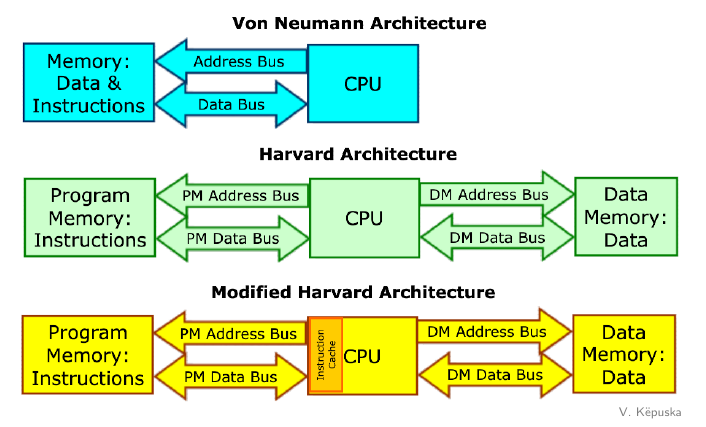
\includegraphics[keepaspectratio, width=\textwidth,height=0.9\textheight-4\baselineskip]{img/200_vonneumann.png}
      \end{center}
      \caption{Von Neumann and Harvard architectures.~\autocite{mrupp}}
      \end{figure}
\end{frame}

\begin{frame}{Bus Systems}
\begin{figure}
       \begin{center}
       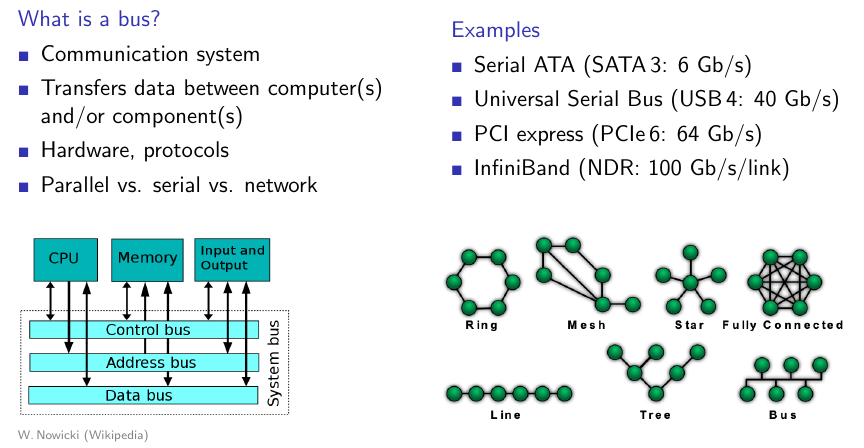
\includegraphics[keepaspectratio, width=\textwidth,height=0.9\textheight-4\baselineskip]{img/201_bus.png}
      \end{center}
      \caption{Bus system and topology examples.~\autocite{mrupp}}
      \end{figure}
\end{frame}

\begin{frame}[allowframebreaks]{Chipset \& Motherboard}
 \begin{figure}
       \begin{center}
       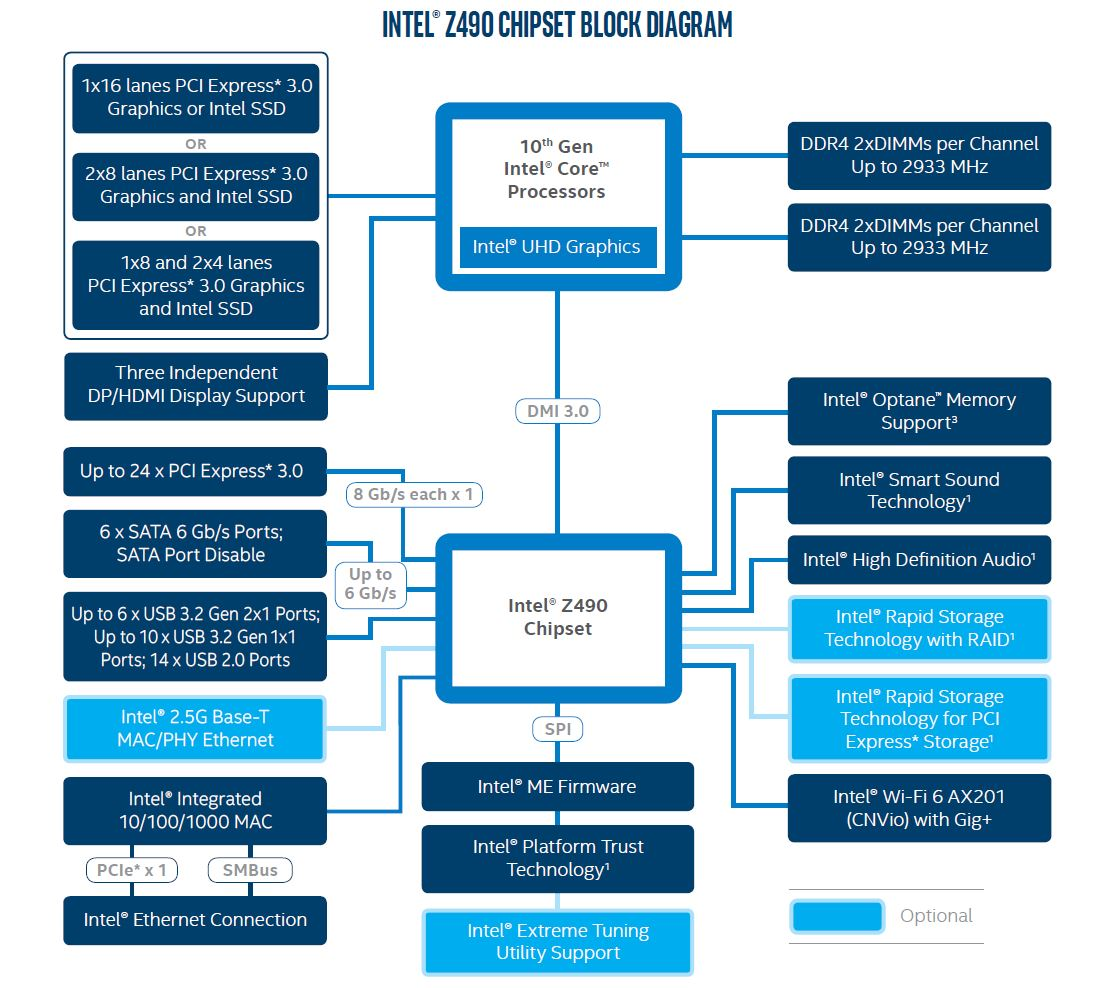
\includegraphics[keepaspectratio, width=\textwidth,height=0.9\textheight-4\baselineskip]{img/202_chipset.jpg}
      \end{center}
      \caption{High Level Diagram of an Intel chipset.~\autocite{intel}}
      \end{figure}
      \framebreak
      \begin{figure}
       \begin{center}
       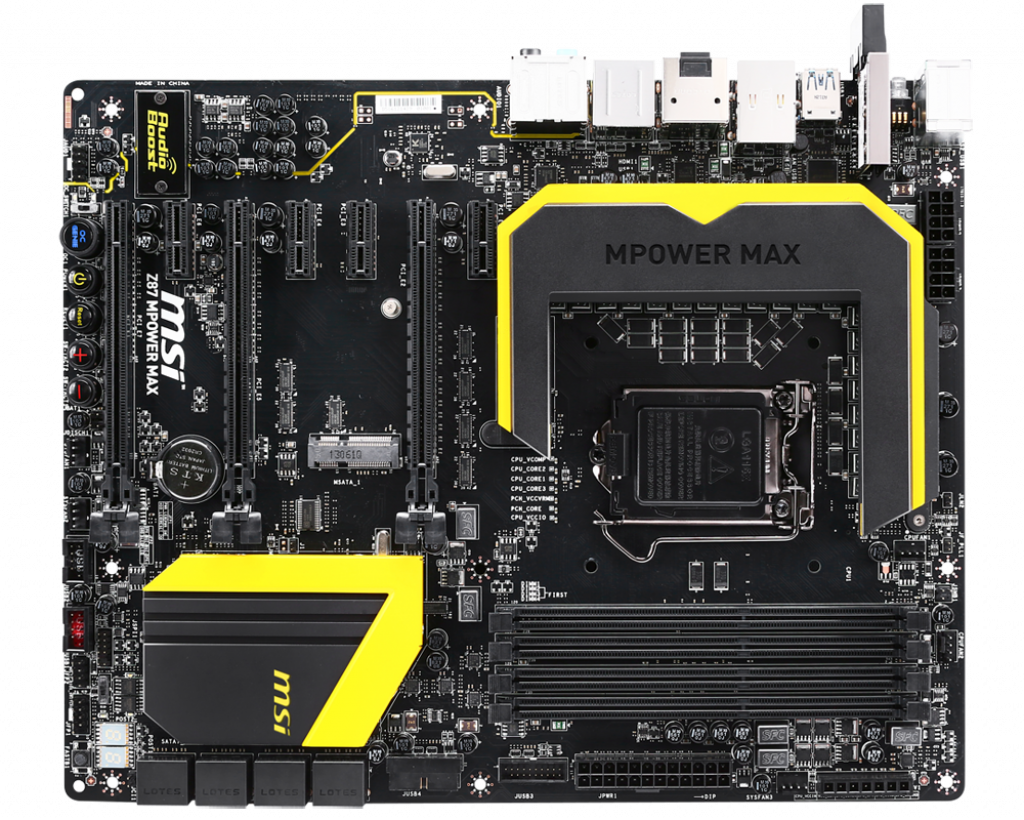
\includegraphics[keepaspectratio, width=\textwidth,height=0.9\textheight-4\baselineskip]{img/201_mboard.png}
      \end{center}
      \caption{A modern moderboard (MSI Z87 MPOWER MAX.~\autocite{msi}}
      \end{figure}
\end{frame}


\begin{frame}[allowframebreaks]{Processors}
\begin{itemize}
 \item 
Exist different processor architectures e.g. \ x64\_86, arm, PowerPC, $\dots$ \\
\item MMU $\equiv$ IMC
\end{itemize}
\begin{figure}
       \begin{center}
       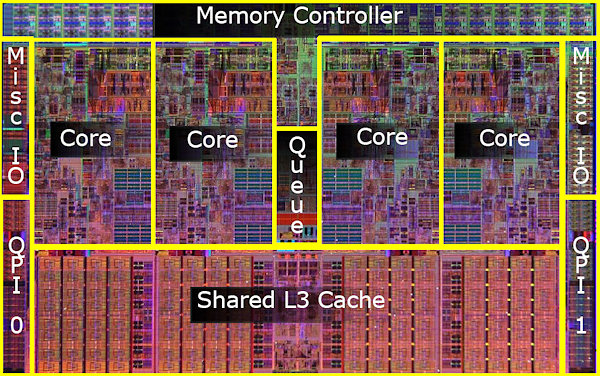
\includegraphics[keepaspectratio, width=\textwidth,height=0.6\textheight-4\baselineskip]{img/203_Cpu-diagram.jpg}
      \end{center}
      \caption{Picture of an i7.~\autocite{crate}}
      \end{figure}
\framebreak
      \begin{figure}
       \begin{center}
       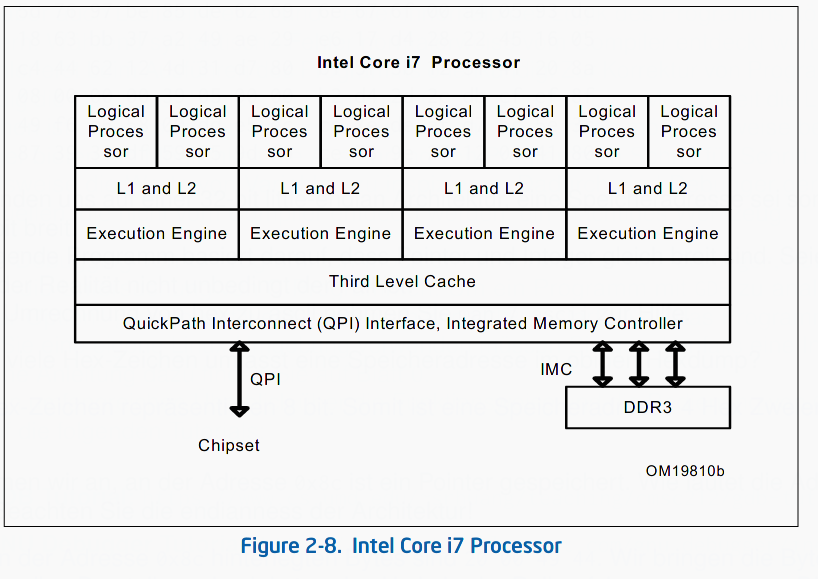
\includegraphics[keepaspectratio, width=\textwidth,height=0.8\textheight-4\baselineskip]{img/203_i7.png}
      \end{center}
      \caption{High Level Diagram of an Intel i7 processor.~\autocite{intel}}
      \end{figure}
      \framebreak
      \begin{figure}
       \begin{center}
       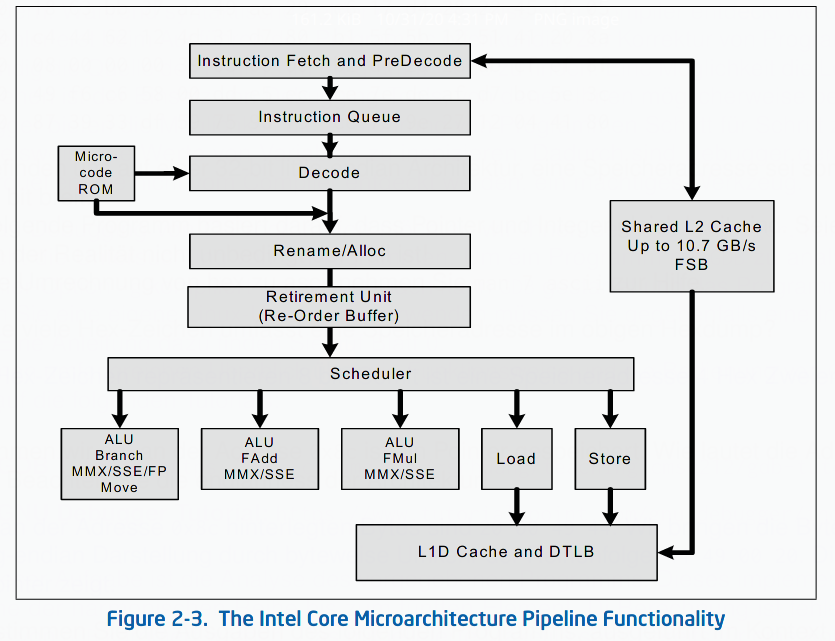
\includegraphics[keepaspectratio, width=\textwidth,height=0.9\textheight-4\baselineskip]{img/204_execution_engine_i7.png}
      \end{center}
      \caption{High Level Diagram of an Intel execution engine.~\autocite{intel}}
      \end{figure}
      \framebreak
      \begin{figure}
       \begin{center}
       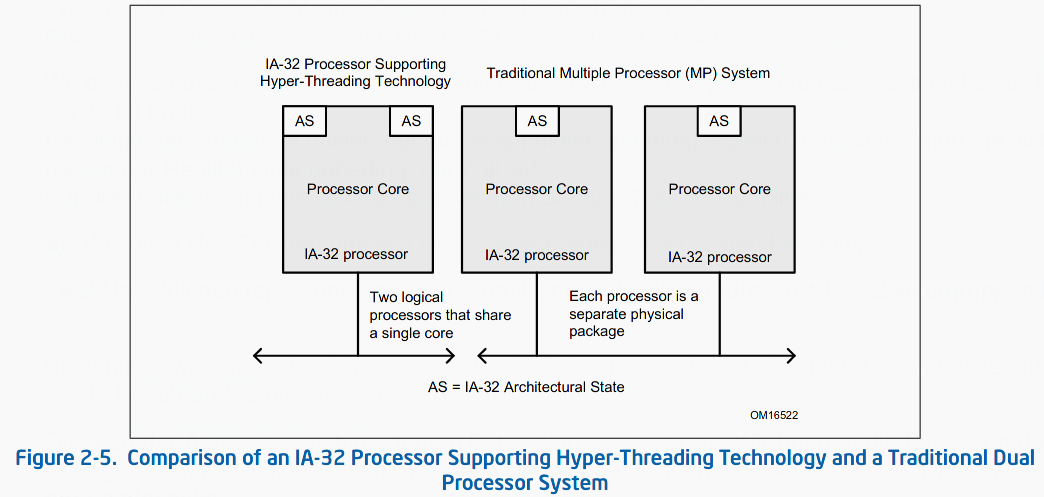
\includegraphics[keepaspectratio, width=\textwidth,height=0.9\textheight-4\baselineskip]{img/205_hyperthreadding.png}
      \end{center}
      \caption{Intel's Hyperthreadding compared to actual cores.~\autocite{intel}}
      \end{figure}
      \framebreak
      \begin{figure}
       \begin{center}
       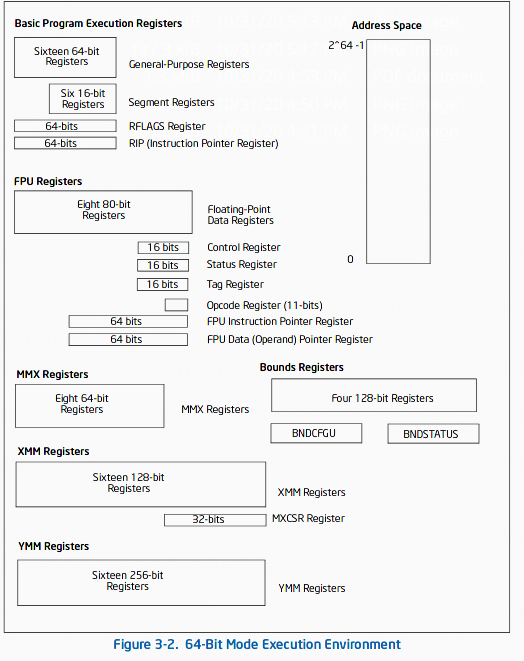
\includegraphics[keepaspectratio, width=\textwidth,height=0.9\textheight-4\baselineskip]{img/206_registers.png}
      \end{center}
      \caption{Registers on an x64 CPU.~\autocite{intel}}
      \end{figure}
\end{frame}

\begin{frame}[allowframebreaks]{Random Access Memory}
\begin{itemize}
 \item Most common: Double Data Rate Synchronous Dynamic Random Access Memory
 \item Current market technology: DDR4-SDRAM
 \item Bus/IO clock defines data rate (w/o prefetch): 
     \[ \text{IO frequency } \cdot 2 \text{ DDR } \cdot 64 \text{ (bus width) } \cdot \frac{1}{8}\text{ (bits per byte) } \] 
        \[= \text{ effective data rate in bytes per seconds} \]
 \item  8-time prefetch enables theoretically 8 times the data rate (if all prefetches hit). 
 \framebreak
 \item Realistically the latencies set the actual memory performance:
 \begin{enumerate}
  \item Column Acess Strobe (CAS) --- latency: How many cycles to serve data.
  \item row to column access time (tRCD): memory cell is read via row and column signals. Constant delay between signals is tRCD.
  \item precharge delay (tPR): Time to deliver necessary voltage for access
  \item Row active time (tRAS): Theoretically CAS + tRP + safety delay; amount of cycles to access cell after previous op.
 \end{enumerate}
\end{itemize}
\framebreak
\begin{figure}
       \begin{center}
       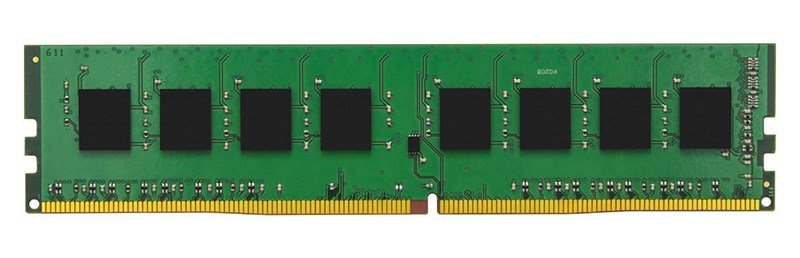
\includegraphics[keepaspectratio, width=\textwidth,height=0.9\textheight-4\baselineskip]{img/206_ddr4-ram.jpg}
      \end{center}
      \caption{Picture of a DDR4-SDRAM unit.~\autocite{store}}
      \end{figure}
\end{frame}

\begin{frame}[allowframebreaks]{GPUs}
 \begin{figure}
       \begin{center}
       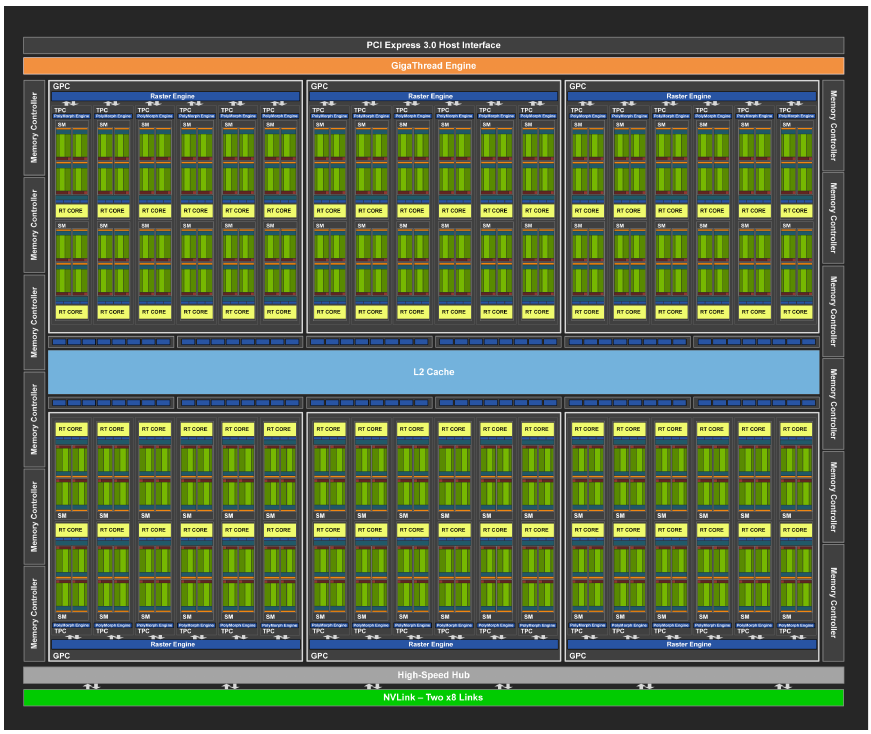
\includegraphics[keepaspectratio, width=\textwidth,height=0.8\textheight-4\baselineskip]{img/209_turing.png}
      \end{center}
      \caption{High level overview of the Nvidia Turing Architecture (here RTX 2080).~\autocite{nvidia}}
      \end{figure}
      \framebreak
      \begin{figure}
       \begin{center}
       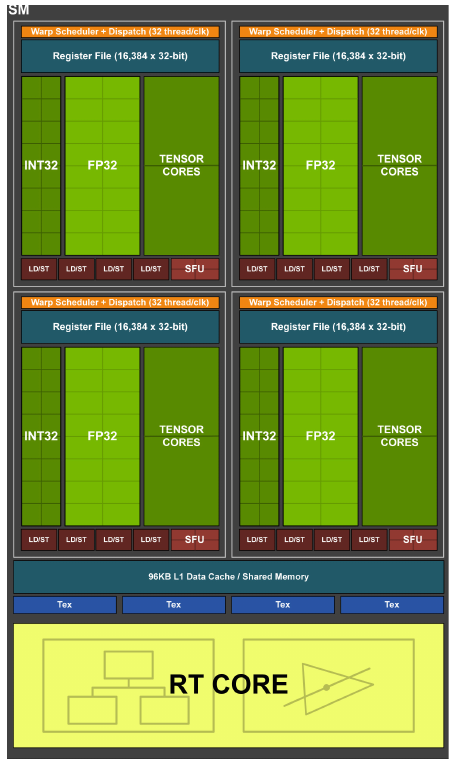
\includegraphics[keepaspectratio, width=\textwidth,height=0.9\textheight-4\baselineskip]{img/210_turing_sm.png}
      \end{center}
      \caption{High level view on a single streaming multiprocessor.~\autocite{nvidia}}
      \end{figure}
\end{frame}


\begin{frame}[allowframebreaks]{IO devices}
 \begin{figure}
       \begin{center}
       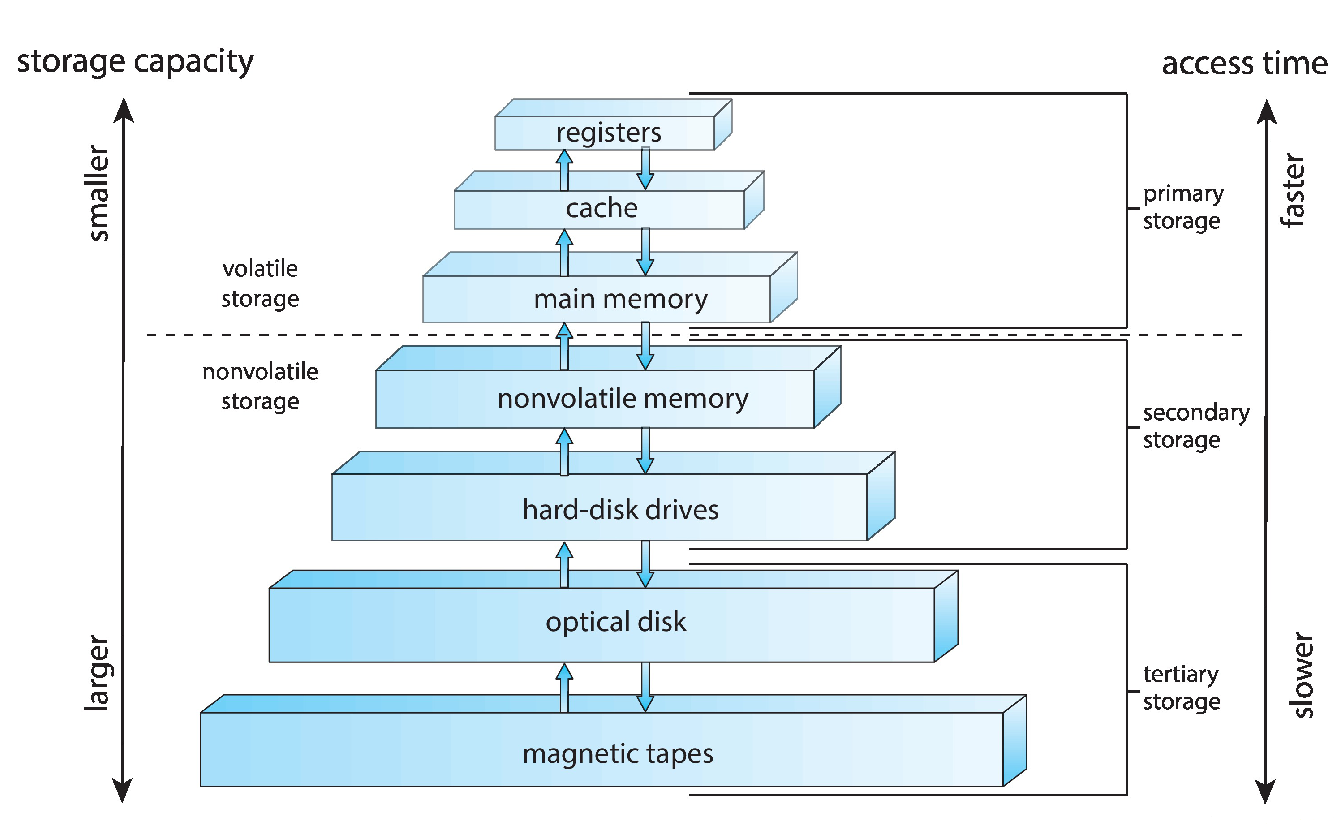
\includegraphics[keepaspectratio, width=\textwidth,height=0.9\textheight-4\baselineskip]{img/207_storage_hierarchy.png}
      \end{center}
      \caption{The Storage hierarchy implemented today.~\autocite{stallings}}
      \end{figure}
      \framebreak
      \begin{figure}
       \begin{center}
       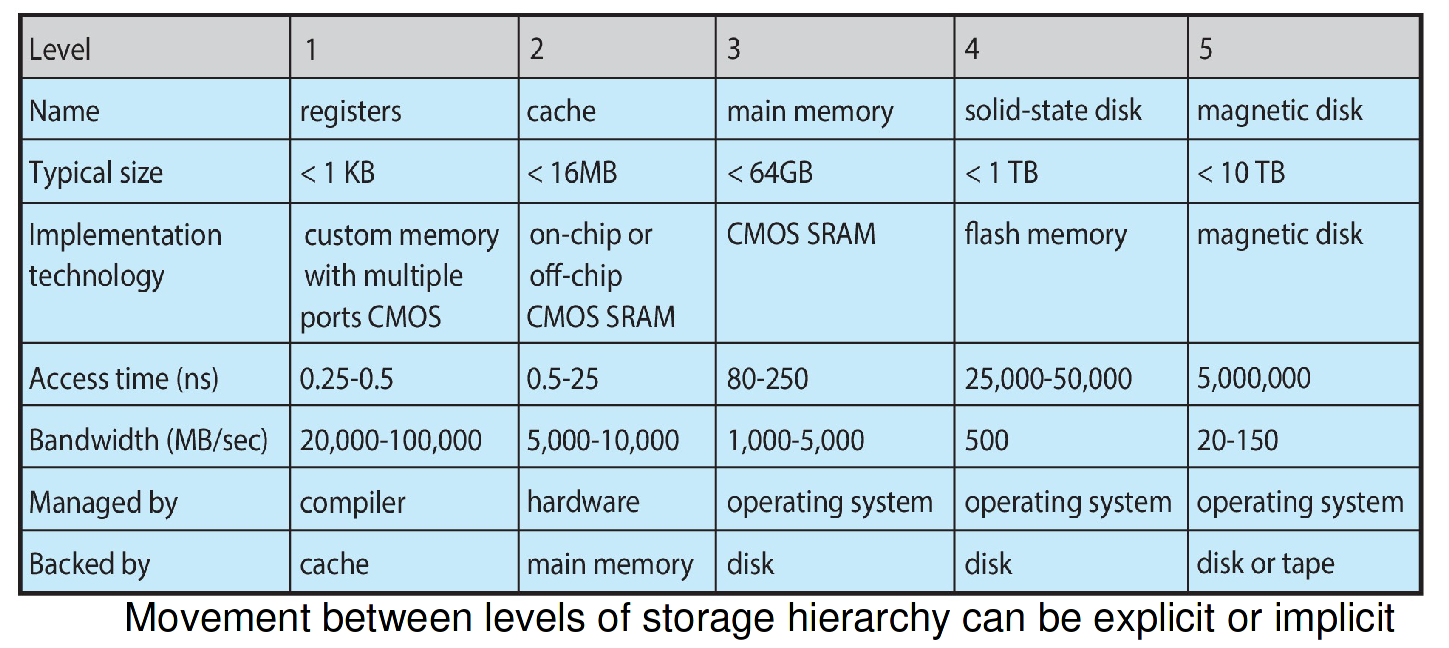
\includegraphics[keepaspectratio, width=\textwidth,height=0.9\textheight-4\baselineskip]{img/207_storage_details.png}
      \end{center}
      \caption{Details on costs and speed.~\autocite{stallings}}
      \end{figure}
      \framebreak
        \begin{figure}
       \begin{center}
       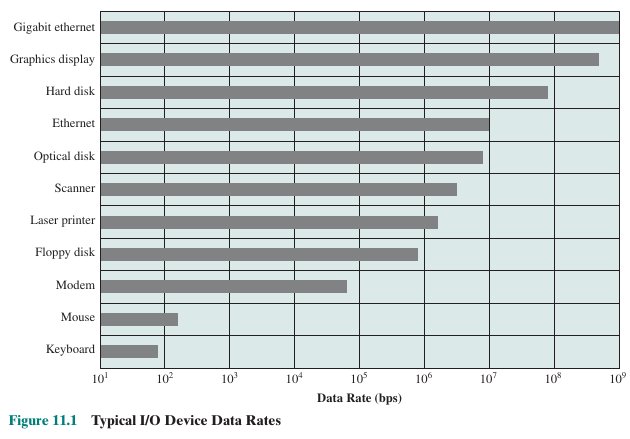
\includegraphics[keepaspectratio, width=\textwidth,height=0.9\textheight-4\baselineskip]{img/208_io_rates.png}
      \end{center}
      \caption{Rates of different IO devices.~\autocite{stallings}}
      \end{figure}
      \framebreak
      \begin{itemize}
       \item Character devices deal with streams of data
       \item Block devices deal with fixed block data
       \item Network devices are special~\autocite{rubini2001linux} (don't show up in \mintinline{bash}{/dev/}, $\dots$)
      \end{itemize}

        \begin{figure}
       \begin{center}
       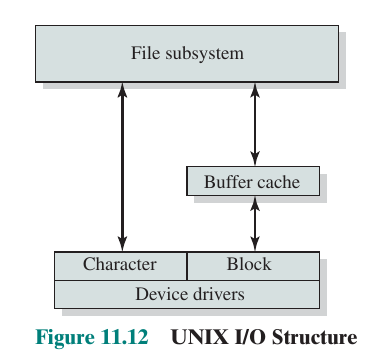
\includegraphics[keepaspectratio, width=\textwidth,height=0.6\textheight-4\baselineskip]{img/211_io_types.png}
      \end{center}
      \caption{The types of devices, as modeled in the UNIX standard.~\autocite{stallings}}
      \end{figure}
\end{frame}


\section{Assignment 1 Primer \&  C Programming }
\begin{frame}{Up next}
    \begin{itemize}
        \item Questions so far? \\
        \item Assignment sheet 1 \\
        \item \mintinline{c}{C} 
    \end{itemize}
    \end{frame}
    
\section{References}
    \begin{frame}[allowframebreaks]
      \frametitle{References}
      \begin{tiny}
      \nocite{*}
      \printbibliography
      \end{tiny}
    \end{frame}


\end{document}
 
